\documentclass{acm_proc_article-sp}

\usepackage{paralist}

\renewcommand{\baselinestretch}{.96}
% \renewcommand{\textfloatsep}{0.7ex}

\usepackage{color}
\newcommand{\todo}[1]{{\small\color{red}[#1]}}

\begin{document}

\title{Robot Learning from Unlabelled Teaching Signals}
% \subtitle{[Extended Abstract]}
\numberofauthors{3}
\author{
%
\alignauthor Jonathan Grizou\\
\affaddr{Flowers Team}\\
       \affaddr{INRIA / ENSTA-Paristech}\\
       \affaddr{France}\\
       \email{\normalsize{jonathan.grizou@inria.fr}}
%
\alignauthor Manuel Lopes \\
\affaddr{Flowers Team}\\
       \affaddr{INRIA / ENSTA-Paristech}\\
       \affaddr{France}\\
       \email{\normalsize{manuel.lopes@inria.fr}}
%
\alignauthor Pierre-Yves Oudeyer\\
	 \affaddr{Flowers Team}\\
       \affaddr{INRIA / ENSTA-Paristech}\\
       \affaddr{France}\\
       \email{\normalsize{pierre-yves.oudeyer@inria.fr}}      
}

\maketitle

\section{Introduction}

Human Robot Interaction (HRI) is the multidisciplinary study of interactions between humans and robots. Researchers in the field investigate how robots properties --- such as embodiment, speech, gesture, facial expression, personality --- can change the behaviour, feelings or attitudes of humans; how robots can produce and recognise communicative acts and how robots and humans can learn from each other \cite{dautenhahn2007socially, fong2003survey}; among others.

Among them \begin{inparaenum}[(a)] \item perception and \item task \end{inparaenum} learning are vastly investigated areas which rely mainly on the machine learning and artificial intelligence community. While impressive results have been obtained in each domain  \cite{argall2009survey, zeng2009survey}, most work considered them separately making important assumptions:
 
 \begin{enumerate}[(a)] 
 
 \item In perceptual learning research applied to HRI, human's communicative signals are learnt to be associated to their respective meanings. Such learning often rely on supervised classification or regression methods, which implies collecting signals samples associated with their respective meanings. This latter requirement implies \textbf{the robot is aware of the communicative goal of the human}.
 
 \item In robot learning from human interaction most work has focused on how to extract statistical task models from human teaching signals \cite{kaplan2002robotic}. Therefore a usual assumption is that \textbf{the robot understands the meanings of human's communicative signals}.
 
 \end{enumerate}
 
Their respective assumptions makes those two lines of research incompatible. On the one hand, working on perceptual learning, i.e.\ learning the signal-to-meaning mapping, requires the robot to know the task. On the other hand, teaching a new task to a robot requires the robot to already know the signal-to-meaning mapping. Consequently it is impossible for a user to interact --- from scratch --- with a robot using his own preferred teaching signals, the user must comply to the use of pre-defined ones. This paper describes a preliminary approach allowing a robot to be instructed a new unknown task by a human using communicative signals initially totally unknown to the robot. In other words, we address the problem of removing the need for calibration.

The question of how a robot can learn to interpret personalised and potentially noisy teaching signals has not been much explored. In a preliminary work \cite{lopes2011simultaneous}, we presented a computational approach addressing this problem by considering a finite space of teaching signals in simulation but requiring to bootstrap the system with known symbols. Later \cite{grizou2013robot}, we released the need for bootstrapping and allow the teacher to use any kind of signal that can be represented as a fixed length feature vector, which is better suited for HRI scenarios.

We provide an intuition on how the algorithm works and report preliminary results.

\section{Intuition}

For the present discussion, we restrain our analysis to scenarios where the user does not actively deliver commands to the robot, but only delivers feedback about actions performed by the robot. Such feedback is given by an unlabelled communicative signals than can be either symbolic, e.g.\ button presses, or represented as a fixed length feature vector, e.g. spoken words. Signals are \textbf{not} converted to a symbolic meaning. The robot needs to actively execute actions to solve the tasks which implies learning the signal-to-meaning association. 

This control can be exemplified for a reaching task, where the user wants the robot to reach a target position unknown at start. The robot performs several actions (e.g.\ moving left or right), and receives unlabelled feedback signals from the user. The feedback signals are generated as a response to the execution of an action in a state according to the true unknown task the user wants to solve. For instance, binary feedback signals simply encode whether the action executed is correct or incorrect according to the user intended task. The key point is that these signals are generated from an underlying model that for binary signals has two different classes.

To solve this problem, we must exploit an other source of information, namely task constraints. Task constraints are properties of the environment that limit the space of possible task, e.g.\ of possible target positions. This set of hypothetic tasks enable us to create a set of hypothetic signal-to-meaning models. Since the right task will assign the right labels to the signals, while the other tasks will gradually mix them, estimating models' likelihood is a good measure to identify the user's intended task. 

\section{Preliminary results}

We construct a small size pick-and-place task with a real robot that has 4 actions available: \textit{rotate left}, \textit{rotate right}, \textit{grasp cube} and \textit{release cube}. This robot is going to be programmed using natural speech with words a priori unknown to the robot. The teacher is facing the robot and chooses a specific arrangement of cube, i.e.\ a specific task, it wants the robot to build. It then decides one word to use as positive feedback and one as negative feedback and starts teaching the robot. Once the robot has understood the first task, using the method presented above, it has also understood the signal-to-meaning model. We can freeze the corresponding classifier and start learning a new task.

\begin{figure}[!h]
	\centering
		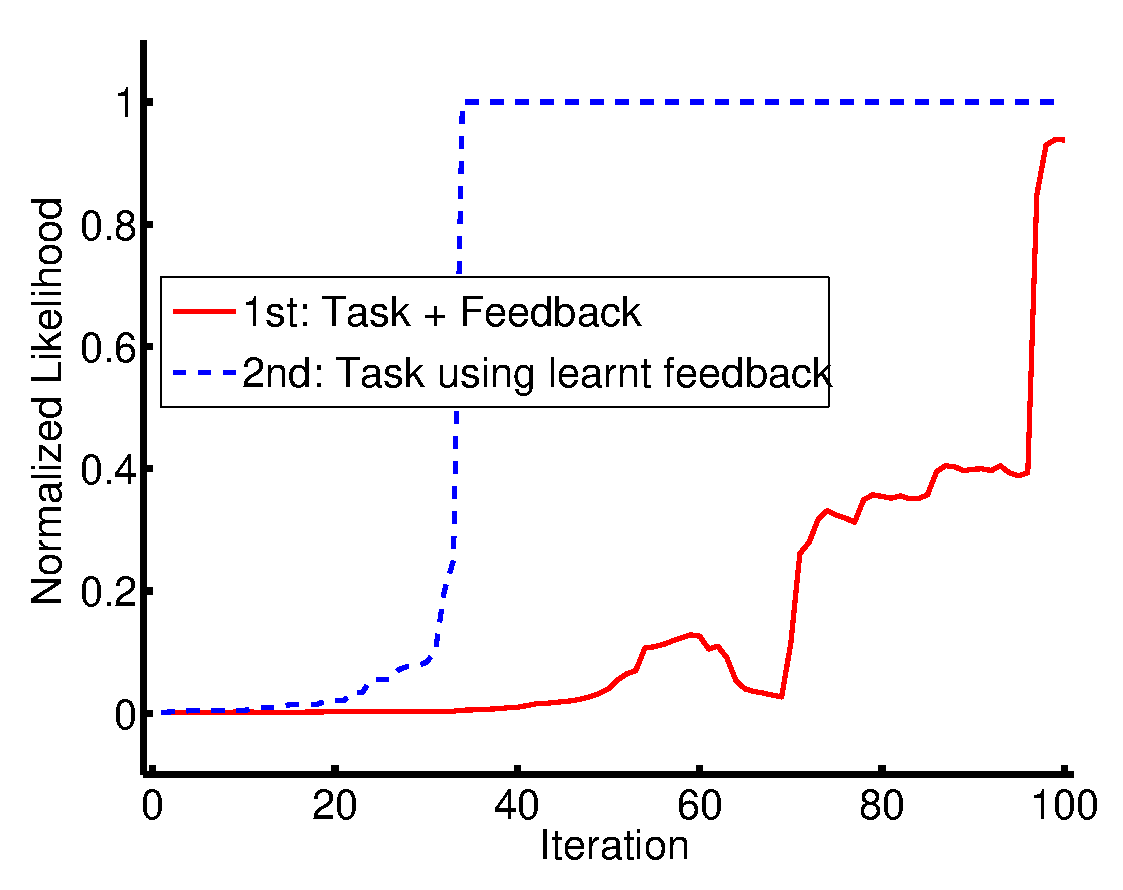
\includegraphics[width=0.8\columnwidth]{foo/real}
	\caption{Evolution of the probability of the taught task. 1) The robot learns a task from unlabelled speech feedback. 2) By freezing the classifier corresponding to the first task, the user teaches the robot a new task faster.}
	\label{Real}
\end{figure}

Fig.~\ref{Real} shows results from this setting. In the first run it takes about 100 iterations for the robot to learn both the task and the signal-to-meaning mapping. Whereas in the second run, when reusing knowledge from the first one, the robot is able to learn a new task faster, in about 30 iterations, meaning that it has well found the two clusters in our feature space as well as the mapping to their corresponding meanings.

\section{Limitations and perspectives}

We presented a new approach for HRI which enables a user to use his own preferred teaching signals when interacting with a robot, e.g. using his own language or defining his own finger movements. The claim that it would be more intuitive or natural to interact with a robot this way is far from being obvious and should be tested with care. When interacting with machine, including robots, we are often, if not always, told how to use them. Do people want to have an open-ended choice about how to interact with machines? Would they be more efficient? Investigating such question is part of our future work.

Our method remove the necessity of a calibration phase. Among the many application requiring calibration, Brain Computer Interaction (BCI) is one of the most challenging. We are currently investigating in this direction \cite{grizou2013zero}. BCI has the advantage to make obvious the fact that we cannot ask the user to comply to the use of pre-defined signals.

An important assumption of our method is that it is possible to define a finite --- and reasonable --- set of task hypothesis. This assumption is limiting for many theoretical problems but many useful real word application can still benefit from it. An eligible scenario is the problem of grasping, on a table, one object among a finite set of objects. In this scenario the set of hypothesis consist of all the objects on the table.

While this is not the main target, the work presented in this paper is also relevant with regards to infant social development and learning, as well as in adult mutual adaptation of social cues. This has been the subject of experiments in experimental semiotics \cite{galantucci2009experimental}, such as in the work of Griffiths et al. \cite{griffiths2012bottom} who conducted an experiment with human learners learning the meaning of unknown symbolic teaching signals. An innovative direction would be to embed the algorithmic principles introduced in this paper for experimental linguistics studies.

\section*{Acknowledgement}
Work (partially) supported by INRIA, Conseil R\'egional \\
d'Aquitaine and the ERC grant EXPLORERS 24007.

\bibliographystyle{abbrv}
\bibliography{hripioneers2014} 

\end{document}